%Exercise 8.1 prob 47
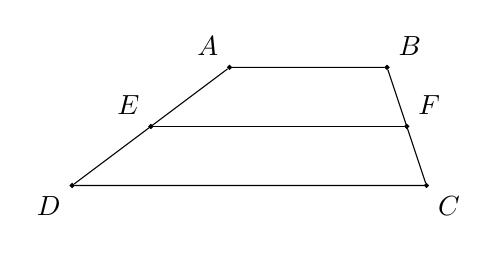
\begin{tikzpicture}
[scale=0.5,>=stealth,point/.style={draw,circle,fill = black,inner sep=0.5pt},]
%\tikzset{shift={(-3,0)}}
%Triangle sides
\def\a{4}
\def\c{9}
\def\d{5}
\def\h{3}
\def\k{1.5}
%\def\c{7.5}

%Labeling points
\node (D) at (0,0)[point,label=below left:$D$] {};
\node (B) at (8,\h )[point,label=above right:$B$] {};
\node (C) at (\c, 0)[point,label=below right:$C$] {};
\node (E) at (2, \k)[point,label=above left:$E$] {};
\node (F) at (8.5, \k)[point,label=above right:$F$] {};
%\node (M) at (4, \k)[point,label=below right:$M$] {};
%\node (N) at (8, \k)[point,label=below right:$N$] {};
%\node (X) at (4, 0)[point,label=below right:$X$] {};
%%node (Y) at (8, 0)[point,label=below right:$Y$] {};
\node (A) at (4,\h)[point,label=above left:$A$] {};
%A



%Drawing parallelogram ABCD
\draw (A) -- (B) --  (C) --(D)--(A);
\draw (E) --(F);
%\draw (B) --(Y);



%
\end{tikzpicture}

